%%%%%%%%%%%%%%%%%%%%%%%%%%%%%%%%%%%%%%%%%%%%%%%%%%%%%%%%%%%%%%%%%%%%%%%%%%%%%%%
% Chapter 2: Descripción de la aplicación: ChefManagement
%%%%%%%%%%%%%%%%%%%%%%%%%%%%%%%%%%%%%%%%%%%%%%%%%%%%%%%%%%%%%%%%%%%%%%%%%%%%%%%

En el capítulo anterior~\ref{chapter:intro} se ha introducido tanto los antecedentes como se describió brevemente la aplicación. En este capítulo explicaremos toda las funcionalidades y sus características con detalle. \\

Partimos de qué tipo de aplicación queremos crear. Se trata de desarrollar un software que ayude a las personas a gestionar el costo de producción de las recetas, dependiendo del precio de sus ingredientes y el número de raciones. Ésta se llamará \textbf{ChefManagement} y sus características iniciales son:
\begin{itemize}
	\item Crear, ver, editar y eliminar recetas.
	\item Listar todas las recetas.
	\item Crear backup de las recetas y cargarlo si es necesario.
	\item Calcular el precio de una determinada receta para un determinado número de comensales.
\end{itemize}

Para esta primera versión, además de ser capaz de realizar esta serie de tareas, debe  cumplir con las necesidades y espectativas del usuario y facilitar su interacción con la aplicación. Éstos son sus requisitos iniciales:
\begin{itemize}
	\item Dos entornos de producción: la aplicación puede ser usada desde dos nubes diferentes.
	\item Tener en cuenta aspectos de usablidad: adaptación, entendimiento y facilidad de uso.
	\item Importar y exportar archivos en formato json: almacenar copias de las recetas en el equipo cliente y restaurarlas si es necesario.
	\item Accesso mediante registro o haciendo uso de APIs de distintas redes sociales como Google+ o Facebook. Hay que facilitar el acceso a los usuarios.
\end{itemize}

Tanto las características comos los requisitos de la aplicación serán aplicadas a la versión 1.0, pudiendo ser mejorados o añadidos más en futuras versiones~\ref{chapter:conclusiones}.

\vspace*{0.2in}
\section{Acceso a la aplicación}\label{cap.2.1}

Para usar esta aplicación podemos acceder directamente a sus entornos de producción:
\begin{itemize}
	\item \href{http://chefmanagement.herokuapp.com/}{Despliegue en Heroku}
	\item \href{http://chefmanagement-esit.rhcloud.com/}{Despliegue en OpenShift}
\end{itemize}

O bien acceder al \href{https://github.com/alu0100207385/ChefManagement}{repositorio} de la aplicación (se trata de licencia libre y código abierto) y seguir las instrucciones de instalación. \\

Una vez en la aplicación encontraremos una pantalla inicial de acceso, que nos permite acceder usando redes sociales, en este caso Google+ y Facebook. Esto es posible gracias al uso de su API (o interfaz de programación de aplicaciones) correspondiente, la cual es un conjunto de funciones o métodos que ofrece una librería para ser utilizado por otro software. En otras palabras, el equipo de desarrollo de Facebook crea esta herramienta para que otras aplicaciones, como Chefmanagement puedan hacer uso de ella. Esto tiene ventajas importantes como la seguridad, desde el punto de vista de desarrollo de software y la comodidad para los usuarios finales. \\

\begin{figure}[H]
	\centering
	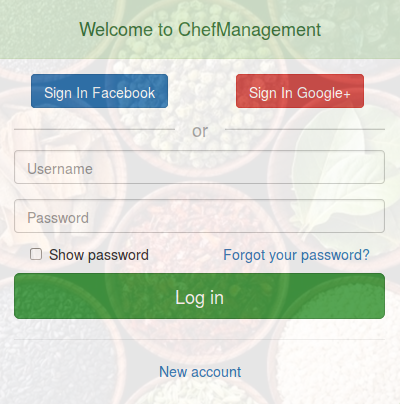
\includegraphics[width=8cm]{./images/chefmanagement-root.png}
	\caption{Acceso a la aplicación} \label{fig:chefmanagement-root}
\end{figure}

Además existe la opción de validarnos en la aplicación, una vez que se haya completado el registro. Si el usuario de entrada o contraseña fueran incorrectos la aplicación lo notificaría. En caso de pérdida de contraseña podemos solicitar una nueva accediendo al enlace \emph{Forgot your password?} y proporcionar nuestro nombre de usuario. Posteriormente puede modificarse la nueva contraseña en opciones~\ref{sec:cap.2.5}.

\begin{figure}[H]
	\centering
	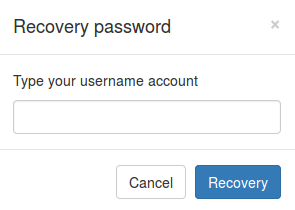
\includegraphics[width=8cm]{./images/chefmanagement-recovery.png}
	\caption{Recuperar contraseña} \label{fig:chefmanagement-recovery}
\end{figure}

Para registarse accedemos a través del enlace \emph{New account}. En caso de cualquier problema durante el proceso de registro, como que el correo o nombre de usuario estén en uso, la aplicación lo notificará al usuario.

\begin{figure}[H]
	\centering
	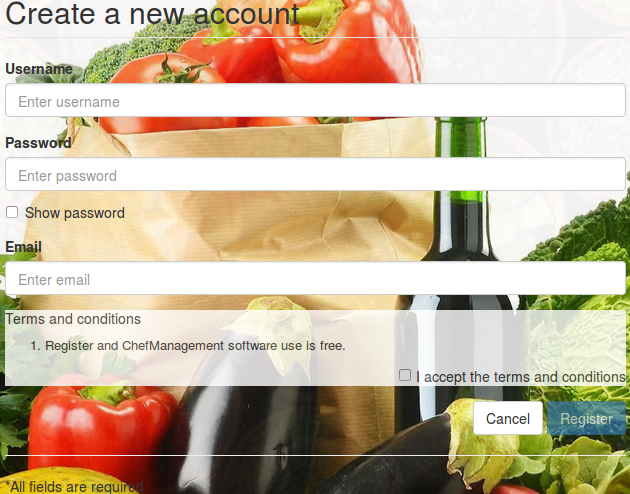
\includegraphics[width=8cm]{./images/chefmanagement-register.png}
	\caption{Registro} \label{fig:chefmanagement-register}
\end{figure}

Una vez dentro de la aplicación accederemos al \emph{home} del usuario. Existe un barra superior donde podemos acceder a la configuración y salir de la aplicación (Log out). También encontramos un menú lateral el cual facilita la interacción del usuario con la aplicación y ayudar a moverse y gestionar las distintas tareas. Por defecto, cuando accedemos a la aplicación, en \emph{home} se nos despliega la lista de recetas creadas por ese usuario. Las opciones del menú son las siguientes:

\begin{itemize}
	\item Recipe list: muestra el listado de recetas del usuario. Podemos acceder, editar y borrar recetas a través de esta lista.
	\item Recipe calculator: calcula el costo de producción de una receta y sus ingredientes para una determinada receta y raciones.
	\item New recipe: crea una nueva receta.
	\item Import: carga una copia de seguridad de las recetas del usuario.
	\item Export: almacena en el equipo local una copa de seguridad de las recetas del usuario.
\end{itemize}


\vspace*{0.2in}
\section{Crear recetas}\label{cap.2.2}

Para acceder a crear receta, nos situamos en el menú lateral y pinchamos en \textbf{New recipe}. Esto nos llevará a una nueva ventana, la cual presentará un formulario con una serie de campos que se detallan a continuación:

\begin{itemize}
	\item Name: es un campo obligatorio y clave primaria en la bbdd. Nombre de la receta.
	\item Rations: Numero de raciones para crear esa receta. Este campo es muy importante ya que se tomará como referencia para el cálculo de recetas dado un determinado número de platos.
	\item Cost: es un campo de lectura, se calcula acutomáticamente con cada ingrediente.
	\item Ration cost: relación entre el coste de la receta y el número de raciones.
	\item Order: campo que sirve como etiqueta. Indica si se trata de un primer o segundo plato, un postre, etc.
	\item Type: segundo campo de etiqueta. Nos da información sobre el tipo de comida: snack, comida casera y otros.
	\item Nivel: nivel de dificultad de producción de la receta.
	\item Time: horas y minutos que se estima que lleva preparar esa receta.
	\item Vegan: indica si la receta es apta para vegetarianos.
	\item Allergens: campo de texto para introducir alimentos que puedan producir alergias.
	\item Origin: información sobre el país originario de la receta.
\end{itemize}

Una vez completado podemos guardar la receta con el botón \textbf{Save recipe} o cancelar el proceso y volver a \emph{home}. Si guardamos la receta el sistema notificará de su registro en la bbdd y abrirá nuevos campos: 

\begin{itemize}
	\item Un área de texto desplegable que se utiliza para escribir las instrucciones de la receta. He utilizado la herramienta \href{http://ckeditor.com/}{ckeditor} para integrarla en la aplicación-
	\item Ingredientes, que puede ser:
		\begin{itemize}
			\item Un \textbf{nuevo ingrediente} creador por el usuario. Campos:
				\begin{itemize}
					\item Nombre del ingrediente
					\item Cantidad: puede ser: peso, volumen o una determinada unidad.
					\item Precio en relación con su cantidad
					\item El porcentaje de merma o pérdida del ingrediente durante su preparación.
				\end{itemize}
			\item \textbf{Una receta} ya creada por el usuario. De forma que las recetas puedan servir de base para crear otras, por ejemplo, la salsa de tomate es una receta que se puede usar en otras. Si una receta usa otra, la primera no puede ser usada para crear otra y no aparecerá como opción en este apartado.
		\end{itemize}
\end{itemize}

A medida que vayamos incluyendo ingredientes a la receta, en el margen lateral derecho se desplegará una lista informativa de la receta con los ingredientes agregados hasta el momento.

\vspace*{0.2in}
\section{Editar y eliminar recetas}\label{cap.2.3}

Desde el listado de recetas podemos editar o eliminar según nuestras necesidades. Para ello pinchamos en una determinada receta y accederemos a toda la información de la receta. Esta opción es de sólo lectura. En la parte superior derecha encontramos los iconos para eliminar y editar la receta. \\

Para eliminar la receta pulsamos el botón de eliminar. El programa pedirá la confirmación para eliminarla. Una vez eliminada no se puede recuperar. Las recetas que sirven de base a otras no pueden ser eliminadas hasta que no se rompa este vínculo, para ello debemos entrar en el modo edición. \\

Si pulsamos en edición, nos llevará a una nueva pantalla donde podemos editar todos los campos de la receta (excepto el nombre y los costos que se calculan automáticamente). Podemos añadir nuevos ingredientes, editar o borrar los actuales o bien borrar \emph{recetas base} (en futuras aplicaciones se recomienda poder añadir \emph{recetas bases}). Así mismo podemos editar las instrucciones de la receta. \\

\vspace*{0.2in}
\section{Calculadora}\label{cap.2.4}

Esta opción nos permite elegir entre el listado de recetas del usuario. Una vez hecho esto seleccionamos el número de raciones que queremos producir y pulsamos en calcular. Se mostrará una tabla resultante con el listado de ingredientes, sus cantidades para las raciones seleccionadas y su precio. De la misma forma se mostrarán las \emph{recetas bases} si contiene alguna y por último el precio de producción final. \\

A modo de información adicional se muestra las instrucciones de la \textbf{receta original}.

\vspace*{0.2in}
\section{Importar y exportar}\label{cap.2.5}

Estas opciones nos permiten crear y cargar una copia de seguridad de las recetas y sus ingredientes del usuario. Para crear una copia, seleccionamos la opción \textbf{Export} del menú lateral. Se mostrará un campo de texto para elegir el nombre del archivo, (por defecto \emph{recipe}) el cual podemos editar y pulsamos en crear. Se comprueba si la cadena introducida contiene caracteres inválidos, en caso contrario se notifica al usuario la operación exitosa y se descarga el archivo al equipo local en formato \textbf{json}. \\

Por otro lado, está la opción de cargar la copia de seguridad. Para ello pulsamos en la opción \textbf{Import}, nos permitirá seleccionar un archivo solo válido en formato json. Una vez seleccionado pulsamos en cargar, en caso de error, la aplicación lo notificará con un mensaje, y si el archivo se ha cargado correctamente nos redirige a \emph{home} con el listado de recetas. Hay que tener en cuenta que si cargamos una copia de seguridad borrará el contenido actual de recetas para cargar ésta.

\vspace*{0.2in}
\section{Opciones}\label{cap.2.5}

Las opciones se encuentran en la parte derecha de la barra superior de la aplicación. Si pulsamos nos lleva a una nueva pantalla que nos muestra el perfil del usuario. Éste se podrá editar en caso de que el usuario haya accedido mediante registro en la propia aplicación, si accedió vía redes sociales debe acceder a las mismas para editar su perfil. \\

También permite la opción de darse de baja de la aplicación. Ello conlleva el borrado de todas sus recetas de la bbdd.

\vspace*{0.2in}
\section{Diseño de la base de datos}\label{cap.2.6}

El modelo propuesto para esta primera versión atendiendo a los requisitos de la aplicación, es el siguiente:
\begin{itemize}
	\item \textbf{Usuarios (User):} Se trata del modelo base y del que depende la gestión del resto. Sus campos son: \emph{username}, \emph{email}, \emph{password} y \emph{network}. Siendo \emph{username} y \emph{email} sus claves primarias. La contraseña y correo del usuario pueden ser editados siempre y cuando no se haya accedido a la aplicación vía Google+ o Facebook.

	\begin{figure}[H]
		\centering
		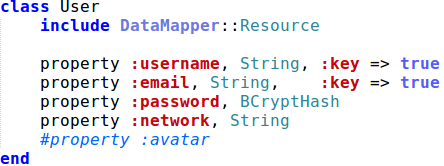
\includegraphics[width=7cm]{./images/chefmanagement-model-user.png}
		\caption{Modelo usuario} \label{fig:chefmanagement-model-user}
	\end{figure}

	\item \textbf{Recetas (Recipe):} Este modelo contiene información sobre la receta creada por un determinado usuario. Establece la relación con la clase Usuario, del que depende de uno a muchos (1:M) y con las clases ingredientes y recetas base, cuya relación es en ambos casos de 1:M. Tiene muchos campos, de los que cabe destacar: \emph{name}, nombre de la receta y clave primaria; \emph{nration}, campo requerido y que indica el número de platos, y \emph{username} que es el autor de la receta. 	Sus relaciones son: una receta puede tener varios ingredientes (clase Ingredients) o varias recetas base (clase Recipe2).

	\begin{figure}[H]
		\centering
		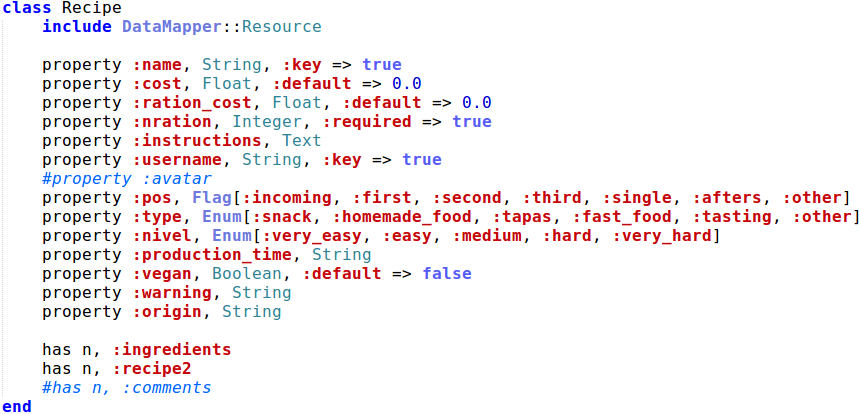
\includegraphics[width=13cm]{./images/chefmanagement-model-recipe.png}
		\caption{Modelo receta} \label{fig:chefmanagement-model-recipe}
	\end{figure}

	\item \textbf{Ingredientes (Ingredient):} Se trata de los ingredientes para cada receta. Por lo tanto depende de la clase receta con una relación de 1:M. Sus campos más importantes son su \emph{id} (clave primaria), \emph{name} que es el nombre del ingrediente y \emph{cost} que corresponde a su coste, siendo estos dos último campos requeridos.

	\begin{figure}[H]
		\centering
		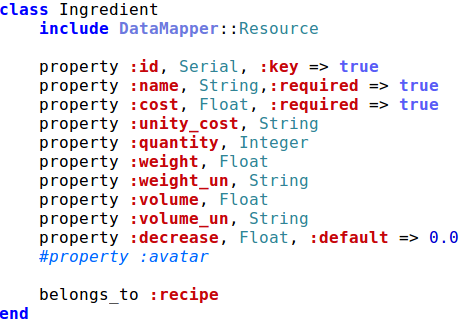
\includegraphics[width=8cm]{./images/chefmanagement-model-ingredient.png}
		\caption{Modelo ingrediente} \label{fig:chefmanagement-model-inredient}
	\end{figure}

	\item \textbf{Recetas base (Recipe2):} Esta clase es una extensión de recipe, que sirve para identificar las recetas usadas como ingredientes en otras, esto es una receta base. Su relación con la clase receta se presenta de 1:M.

	\begin{figure}[H]
		\centering
		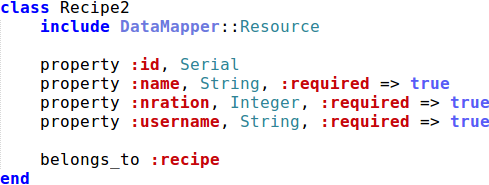
\includegraphics[width=9cm]{./images/chefmanagement-model-recipe2.png}
		\caption{Recetas base} \label{fig:chefmanagement-model-recipe2}
	\end{figure}

\end{itemize}

Los cambios producidos en una clase puede implicar la modificación de las clases con las que está relacionada. Por ejemplo, si se elimina un usuario, se debe eliminar sus recetas y en consecuencia los ingredientes de esa receta. El modelo propuesto se ha diseñado de tal forma que sea capaz de realizar todas las acciones del CRUD, acrónimo de \textbf{C}rear, \textbf{O}btener, \textbf{A}ctualizar y \textbf{B}orrar (Create, Read, Update and Delete) para cada clase. \\

Puede ver con detalle el código fuente del modelo de la aplicación en \href{https://github.com/alu0100207385/ChefManagement/blob/master/app/models/model.rb}{model.rb}.
